\documentclass{aiaa-tc}

%\usepackage[margin=1.0in]{geometry}
\usepackage{fullpage}
\usepackage{graphicx}
\usepackage{bm} %required for bold in math mode for greek symbols
\usepackage{amsmath} %for bmatrix
\usepackage{amsfonts} %for math script font
\usepackage{url} %for website citations

\usepackage[space]{grffile} %for filepaths with spaces
\usepackage[mathscr]{euscript} % for scripty L1 symbol

%define degree symbol:
\newcommand{\degree}{\ensuremath{^\circ}}

\newcommand{\fr}[1]{$#1^+$} %command to write a reference frame
\newcommand{\br}[2]{[#1]_{#2}} %bracket operator with subscript
\newcommand{\tvect}[3]{\begin{bmatrix}#1\\#2\\#3\end{bmatrix}}% 3 x 1 vector
\newcommand{\tvecth}[3]{\begin{bmatrix}#1&#2&#3\end{bmatrix}}% 1 x 3 vector
\newcommand{\B}[1]{\textbf{#1}} %bold for regular vectors
\newcommand{\U}[1]{\hat{\textbf{#1}}} %hats and bold for unit vectors
\newcommand{\BG}[1]{{\bm #1}}           % for vectors using greek letters
\newcommand{\ddt}[1]{\frac{d#1}{dt}} %for time derivatives
\newcommand{\ddarg}[2]{\frac{d#1}{d#2}} % for general derivatives
\newcommand{\pparg}[2]{\frac{\partial#1}{\partial#2}} % for general derivatives
\newcommand{\kron}{\otimes} %redefines \kron to produce kronecker product symbol, for convenience
\newcommand{\squig}[1]{\ensuremath{[{}^{\times} #1]}} % cross product matrix operator
\newcommand{\Lone}{\ensuremath{{\mathscr{L}_1}}} % L1 w/ scripty L


\title{ 3D relative attitude cooperative estimation }
\author{Tim Woodbury}

\let\endtitlepage\relax %surpress line break after title page

\begin{document}

\maketitle

The problem of relative attitude estimation between cooperating agents, with no a priori knowledge of the initial state or known common features, is considered. Previous analyses has considered cooperative sequential state estimation between multiple robotic agents for a purely planar scenario. A key assumption in this work has been that each agent can exploit raw workspace feature measurements made by other agents, given that every agent makes and shares an additional measurement of the range and/or bearing to every other agent. From a trivial geometric analysis of planar motion, it is apparent that bearing measurements between any two agents, when fused, allow determination of the relative bearing between the agents. This knowledge of the relative heading allows any cooperating agent to use feature measurements from another agent, without the need to share estimated states and this couple the estimators in an undesireable fashion.

In taking this estimation scheme from 2D to 3D, a major question to address is: under what circumstances, if any, are range-agnostic interagent measurements sufficient to compute or estimate the relative attitude between the two agents? The problem of single-point attitude detemination has received much attention, particularly in the areas of star navigation, and it is well-known that a minimum of \textbf{two} vectors must be measured, each in different reference frames, to determine the relative attitude between the reference frames, for the single-point determination problem. It is assumed, then, that relative attitude cannot simply be determined from two interagent vector measurements alone. However, we consider here the problem of sequential attitude estimation, exploiting fully or partially measured interagent dynamics (in this case, relative angular velocity). It is not clear that the restrictions that apply to the single-point problem will apply to the sequential estimation problem here. The simplest conceivable scenario is analyzed: each agent has measurements from a three-axis gyroscope, and measures the vector to the other agent.

The governing equations between an agent, designated $i$, and a remote agent $j$ that $i$ senses, are now developed. We consider the problem of estimating the attitude of $j$ relative to $i$, parameterized by generic coordinates $\B{q}_{j/i}$. The angular velocities of each agent relative to the inertial frame are $\BG{\omega}_{i/n}$ and $\BG{\omega}_{j/n}$, and each are assumed to be coordinatized in the corresponding agent body-fixed frame when applicable. The time rate of change of the attitude coordinates is simply linear function of the relative angular velocity $\BG{\omega}_{j/i}$, where $[A(\B{q}_{j/i})]$ is a matrix of appropriate dimensions that depends on $\B{q}_{j/i}$ only:

\begin{equation}
\dot{\B{q}}_{j/i} = [A(\B{q}_{j/i})]\BG{\omega}_{j/i}
\label{eq:qji}
\end{equation}

The relative angular velocity in the \fr{j} frame is simply:

\begin{equation}
[\BG{\omega}_{j/i}] = [\BG{\omega}_{j/n}] + [C_{j/i}(\B{q}_{j/i})][\BG{\omega}_{i/n}]
\label{eq:omegaji}
\end{equation}

The unit vector pointing from $i$ to $j$, i.e. the vector measured by agent $i$, is designated $\U{r}_{j/i}$. Again, letting the measurement by each agent be coordinatized in its own body-fixed reference frame, the measurements made by $i$ and $j$ of onw another should be related by:

\begin{equation}
[\U{r}_{i/j}] = -[C_{j/i}(\B{q}_{j/i})][\U{r}_{j/i}]
\label{eq:rijtemp}
\end{equation}

Subtracting the left-hand side of Eq. \ref{eq:rijtemp} from the right-hand side, the measurement equation is obtained. Note that the measurement $\tilde{\B{y}}$ is a function of the estimated attitude $\hat{\B{q}}_{j/i}$:

\begin{equation}
\tilde{\B{y}} = -[C_{j/i}(\hat{\B{q}}_{j/i})][\tilde{\U{r}}_{j/i}] - [\tilde{\U{r}}_{i/j}]
\label{eq:ytilde}
\end{equation}

The expected value of $\tilde{\B{y}}$, of course, is $\hat{\B{y}} = \B{0}$.

\section{ EKF measurement equations and noise model }

\subsection{Measurement vector and linearization}

The attitude coordinates $\B{q}_{j/i}$ are now specified as quaternion and re-designated $\BG{\beta}_{j/i} = \begin{bmatrix}
\beta_0 \\
\BG{\beta}
\end{bmatrix}$ for clarity. This allows the direction cosine matrix $C_{j/i}$ to be written as an explicit function of the coordinates:

\begin{equation}
[C_{j/i}(\BG{\beta}_{j/i})] = \B{I}_{3 \times 3} - 2\beta_0 \BG{\beta}^\times + 2\BG{\beta}^\times\BG{\beta}^\times
\end{equation}

The gradient of the measurement vector $\B{h}$ with respect to the attitude coordinates is now written in terms of $\hat{\BG{\beta}}_{j/i}$:

\begin{equation}
\ddarg{\B{h}}{\hat{\hat{\BG{\beta}}}_{j/i}} = \begin{bmatrix}
2\hat{\BG{\beta}}^\times [\tilde{\B{r}}_{j/i}] & 2\hat{\BG{\beta}}^\times[\tilde{\B{r}}_{j/i}^\times] + 2[\hat{\BG{\beta}}^\times [\tilde{\B{r}}_{j/i}]]^\times - 2\hat{\beta}_0 [\tilde{\B{r}}_{j/i}^\times]
\end{bmatrix}
\label{eq:HlinDef}
\end{equation}

\subsection{Error model and associated covariance matrix}
\label{sec:pointingErrorModel}

The pointing error and associated covariance matrix for each measurement are now considered. Each measured unit vector should be related to the true unit vector by a (hopefully) small rotation about an (unknown) rotation axis. If a reference frame is established whose 1 axis is parallel to the measured unit vector, the error vector to the true unit vector will lie in the 2-3 axis plane of that frame. In that reference frame, then, the measurement covariance is taken to be: $[R_e] = \mathrm{diag} \begin{bmatrix} 0 & \sigma_p^2 & \sigma_p^2
\end{bmatrix}$

The measurement covariance in the associated vehicle body frame is related to $[R_e]$ by a transformation matrix $[C_{b/e}]$:

\begin{equation}
[R_b] = [C_{b/e}][R_e][C_{b/e}]^T
\end{equation}

The cosine matrix $[C_{b/e}]$ is defined from the body frame unit vector measurement and one arbitrary orthogonal vector, chosen by computing the cross product of the measured unit vector with a unit vector whose components are chosen from the uniform distribution on $[-1,1]$. The body-frame covariance $[R_b]$ is independent of the choice of the orthogonal vector.

From the body-frame covariance $[R_b]$, the measurement covariance is now determined from the Jacobian $[J]$ of the output equation with respect to the unit vector. Defining the $6 \times 1$ vector $\tilde{\B{R}} = \begin{bmatrix}
\tilde{\B{r}}_{j/i} \\
\tilde{\B{r}}_{i/j}
\end{bmatrix}$, the Jacobian of $\B{h}$ is:

\begin{equation}
[J] \equiv \ddarg{\B{h}}{\tilde{\B{R}}} = \begin{bmatrix}
-[C_{j/i}] & -\B{I}_{3\times 3}
\end{bmatrix}
\end{equation}

The covariance matrix associated with $\tilde{\B{R}}$, in terms of agent $i$ and $j$'s body frame measurement covariances $[R_i]$ and $[R_j]$, respectively, is $[R_{\tilde{R}}]$:

\begin{equation}
\begin{bmatrix}
[R_{\tilde{R}}] = \begin{bmatrix}
[R_i] & \B{0}_{3\times 3} \\
\B{0}_{3\times 3} & [R_j]
\end{bmatrix}
\end{bmatrix}
\end{equation}

The covariance associated with the measurement vector $\B{h}$ is approximated by $[R_y]$:

\begin{equation}
[R_y] \equiv J[R_{\tilde{R}}]J^T
\end{equation}

The development in this section applies generally to the problem of relative attitude estimation, given the vector measurements between agents assumed. The EKF equations are now fully developed in each section for the particular cases considered.

\section{ First case: Relative attitude estimation with IMU shared }

In this scenario, agents are assumed to have access to current gyroscope measurements from one another. These measurements are used in state propagation. The estimated state is only the quaternion components $\BG{\beta}_{j/i}$, and an additive error is assumed for simplicity. The propagation in this case, derived from Eq. \ref{eq:omegaji}, reduces to:

\begin{align}
[A(\hat{\BG{\beta}}_{j/i})] \equiv \frac{1}{2} \begin{bmatrix}
-\hat{\BG{\beta}}^T \\
\hat{\beta}_0 \B{I}_{3\times 3} + \hat{\BG{\beta}}^\times
\end{bmatrix} \\
\dot{\hat{\BG{\beta}}}_{j/i} = [A(\hat{\BG{\beta}}_{j/i})] [\tilde{\BG{\omega}}_{j/n} - [C_{j/i}(\hat{\BG{\beta}}_{j/i})] \tilde{\BG{\omega}}_{i/n}] + 
\begin{bmatrix}
[A(\hat{\BG{\beta}}_{j/i})] & -[A(\hat{\BG{\beta}}_{j/i})][C_{j/i}(\hat{\BG{\beta}}_{j/i})]
\end{bmatrix} 
\begin{bmatrix}
\B{v}_i \label{eq:quatDerivative}\\
\B{v}_j
\end{bmatrix} \\
\B{v}_i \sim N(0,R_{\omega,i}) \\
\B{v}_j \sim N(0,R_{\omega,j})
\end{align}

The gyroscope noise covariance $[R_{\omega}]$ is assumed to be the same for both agents. The linearized state influence matrix is given from:

\begin{align}
\BG{\omega}_p \equiv \tilde{\BG{\omega}}_{j/n}-\tilde{\BG{\omega}}_{i/n} \\
[F] \equiv \ddarg{\dot{\hat{\BG{\beta}}}_{j/i}}{\hat{\BG{\beta}}_{j/i}} = \frac{1}{2}
\begin{bmatrix}
0 & -\BG{\omega}_p^T \\ \BG{\omega}_p & -\BG{\omega}_p^\times
\end{bmatrix} + \begin{bmatrix}
\B{0}_{1\times 4}\\
2\hat{\beta}_0 \hat{\BG{\beta}}^\times \tilde{\BG{\omega}}_{i/n} & -\hat{\beta}_0^2 \tilde{\BG{\omega}}_{i/n}^\times + [\hat{\BG{\beta}}^\times \hat{\BG{\beta}}^\times \tilde{\BG{\omega}}_{i/n}]^\times + \hat{\BG{\beta}}^\times [\hat{\BG{\beta}}^\times \tilde{\BG{\omega}}_{i/n}]^\times + \hat{\BG{\beta}}^\times \hat{\BG{\beta}}^\times \tilde{\BG{\omega}}_{i/n}^\times 
\end{bmatrix}
\end{align}

The complicated expression for $[F]$ arises due to the product $[A(\hat{\BG{\beta}}_{j/i})][C_{j/i}(\hat{\BG{\beta}}_{j/i})]$. The preceding equations have fully defined the linearized state and process noise influence matrices for the EKF propagation step. Combined with the equations from the prior section, the full estimation problem has been outlined and relevant terms presented.

\subsection{Simulation}

In simulation, agents are initialized randomly in a 10 meter sphere. Each agent flies to a point in the sphere, chosen on the uniform distribution, following polynomial trajectories for position and Euler angles. Agents continue until the simulation time ends. Agents measure unit vectors to one another, and make IMU gyroscopic measurements in their own body frame. Using these two measurements only, both the Extended Kalman Filter (EKF) and Unscented Kalman Filter (UKF) are implemented using the equations developed in the previous section. Filter values are initialized with uniformly distributed initial quaternion components that are subsequently normalized.

Results are discussed briefly, as the primary purpose of this section is to establish the validity of the sequential filter for relative attitude determination in this framework. Results presented are for the UKF, whose performance is consistent with the EKF. Fig. \ref{fig:error_history_w_omega_measured} shows the error history for a 150 second simulation with two agents. The figure demonstrates that the filter is readily able to regulate the relative attitude estimate error. Fig. \ref{fig:estimate_history_w_omega_measured} shows the true and estimated relative attitude quaternion components for the first two seconds of simulation. Despite being initialized randomly, the filter is rapidly able to converge to the truth values.

\begin{figure}[tb!]
\centering
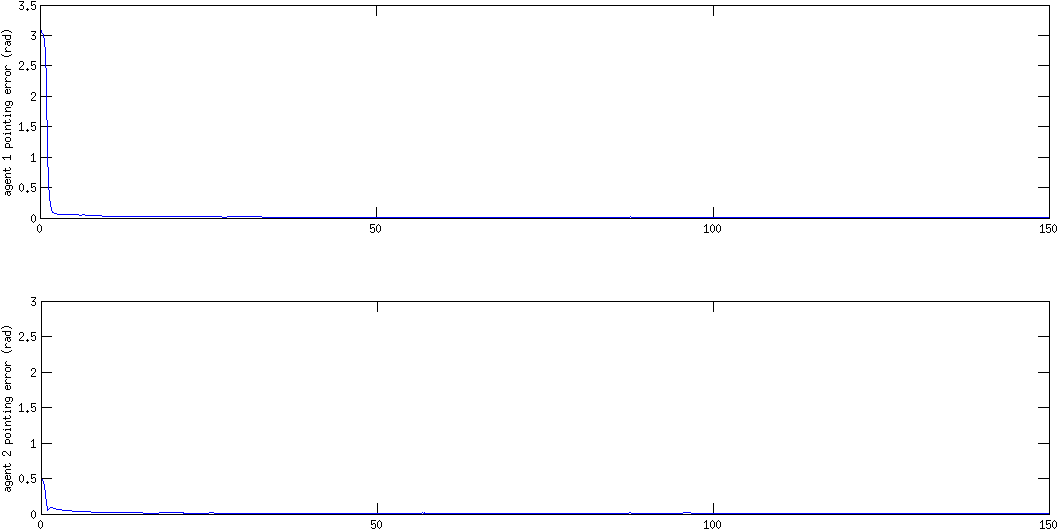
\includegraphics[width=1.0\textwidth]{error_history_w_omega_measured.png}
\caption{Relative heading estimate angular error history.}
\label{fig:error_history_w_omega_measured}
\end{figure}

\begin{figure}[tb!]
\centering
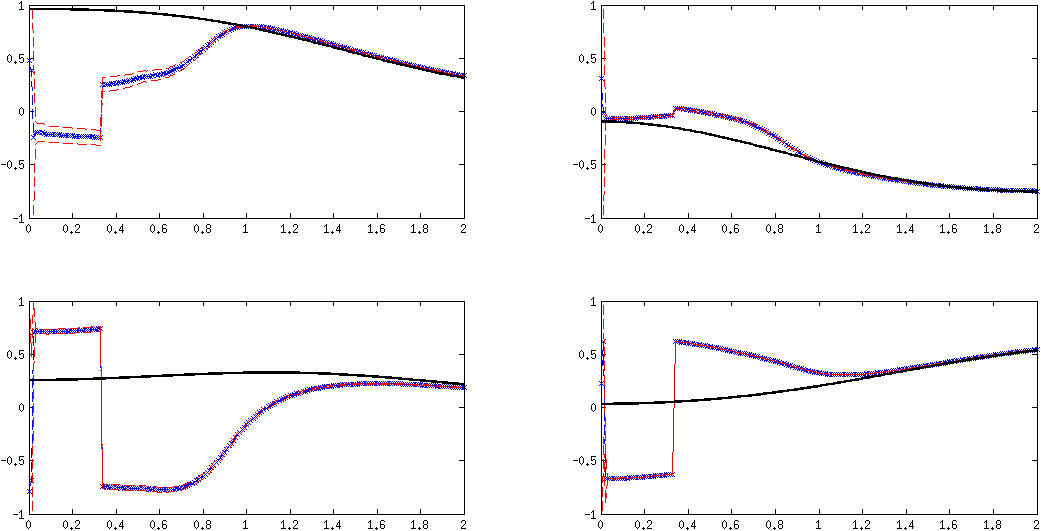
\includegraphics[width=1.0\textwidth]{estimate_history_w_omega_measured.png}
\caption{Relative quaternion estimate and truth for one agent in simulation.}
\label{fig:estimate_history_w_omega_measured}
\end{figure}

\section{Relative attitude estimation without shared IMU - interagent measurements only}

In prior 2D analyses of cooperative estimation, shared IMU data between agents has been treated as a special case, availability of which may be restricted based on agent relative pose and communications limitations. It is highly desireable to have an estimation framework that can enable cooperative SLAM without sharing high-rate IMU data. This section considers the case where both agents measure vectors to the other agent and gyroscopic measurements, but do not share the IMU data.

For this case, the state vector is augmented with an estimated state associated with the other agent's angular velocity. That is, agent $i$'s estimation state vector is augmented with $\br{ \hat{ \BG{\omega} }_{j/n} }{j}$, which is agent $j$'s measured angular velocity in its body-fixed reference frame. The measurement model is not modified, as only the relative attitude affects the expected measurement. In the process model, the estimate $\hat{\BG{\omega}}_{j/n}$ replaces the measured value used in Eq. \ref{eq:quatDerivative}, and the propagation model associated with $\hat{\BG{\omega}}_{j/n}$ is:

\begin{align}
\hat{\dot{\BG{\omega}}}_{j/n} = \B{v}_{\omega} \\
\B{v}_{\omega} \ \in \ N(0,\sigma_{est})
\end{align}

Using the linearized process and measurement models from the previous section, observability analysis can be carried out symbolically to determine if this state parameterization is viable. It can be shown that, after considering the first three terms of the observability matrix, i.e.:

\begin{equation}
[O] = \begin{bmatrix}
H\\
HF\\
H^2F\\
\vdots
\end{bmatrix}
\end{equation}

This matrix is determined numerically to be full rank in general, an exactly sufficient condition for observability for a truly linear system.

\subsection{Simulation}

Numerical simulation of this scenario has proved nonviable. It is possible that performance of the estimator is highly sensitive to the assumed process noise term $\sigma_{est}$ and/or to the interagent vector measurement accuracy. The success of numerical simulation has varied. The pointing error in the relative attitude estimate appears to decrease and increase at different times in the simulation, as though the estimator converges and then diverges. It may be that, as in monocular SLAM, the estimator performance is highly dependent on the interagent motion and cannot achieve good performance for arbitrary relative motion.

\section{Relative attitude estimation without shared IMU - interagent and magnetometer measurement shared}

In the previous section, it was shown that, despite theoretical observability of the relative attitude without IMU sharing, consistently good estimation could not be achieved in simulation for arbitrary interagent relative motion. In this section, the effect of an additional shared vector measurement is considered - in this case, a three-axis magnetometer. In lieu of a magnetometer, cooperating agents might use workspace features simultaneously observed, or (for a larger cohort of vehicles) measurements to other agents as additional measurements.

In the case of magnetometer measurements, each agent is assumed to measure the inertial 1-axis vector in its body-fixed frame. A pointing error is added to this measurement, as in Sec. \ref{sec:pointingErrorModel}. The associated measurement covariance is computed as for the interagent measurement, using an independent noise value based on a magnetometer error $\sigma_m$. The measurement model is altered by appending a measurement of an additional vector. Let $\U{m}$ indicate the vector pointing to magnetic north, i.e. parallel to the inertial 1-axis. The measurement associated with this vector for agent $i$ can be written in a nearly identical fashion to that of Eq. \ref{eq:ytilde}:

\begin{equation}
\tilde{\B{y}} = [C_{j/i}(\hat{\B{q}}_{j/i})]\br{\tilde{\U{m}}}{i} - \br{\tilde{\U{m}}}{j}
\end{equation}

\subsection{Simulation}

Simulation results for this case are promising and consistently show rapid convergence to the true relative attitude. Accurate estimation of the other agent's angular velocity is more difficult, particularly near discontinuities in the agent motion, but in general the true value is well-modelled by the estimate.

\section{Conclusions}

\begin{enumerate}
\item For the case where shared unbiased gyroscope measurements are available to both agents, estimation of the relative attitude is readily achieved.
\item For the case where the remote agent's angular rates are estimated, not shared, estimation of the relative attitude is not achieved for arbitrary interagent motion when agents only have common measurements of the vector pointing to each other.
\item When the remote agent's angular rates are estimated, appending an additional common measurement of any vector in the body reference frames of both agents appears sufficient to achieve accurate estimation of the relative attitude and angular rates.
\end{enumerate}

%\bibliographystyle{plain}

%\bibliography{refs}

\end{document}
